\documentclass[a4paper,12pt]{article}

% Поля страниц
\usepackage[left=2.5cm,right=2.5cm,
top=2cm,bottom=2cm,bindingoffset=0cm]{geometry}

% Рисунки
\usepackage{caption,floatrow}
\usepackage{floatrow,graphicx,calc}
\usepackage{wrapfig}

%Пакет дял таблиц   
\usepackage{multirow} 
\usepackage{array,tabularx,tabulary,booktabs} % Дополнительная работа с таблицами
\usepackage{longtable} 

%Отступ после заголовка    
\usepackage{indentfirst}

%%% Работа с русским языком
\usepackage{cmap}					% поиск в PDF
\usepackage{mathtext} 				% русские буквы в формулах
\usepackage[T2A]{fontenc}			% кодировка
\usepackage[utf8]{inputenc}			% кодировка исходного текста
\usepackage[english,russian]{babel}	% локализация и переносы

%%% Дополнительная работа с математикой
\usepackage{amsmath,amsfonts,amssymb,amsthm,mathtools} % AMS

%% Номера формул
\mathtoolsset{showonlyrefs=true} % Показывать номера только у тех формул, на которые есть \eqref{} в тексте.

\usepackage{icomma} % "Умная" запятая: $0,2$ --- число, $0, 2$ --- перечисление

%% Шрифты
\usepackage{euscript}	 % Шрифт Евклид
\usepackage{mathrsfs} % Красивый матшрифт

%% Перенос знаков в формулах (по Львовскому)
\newcommand*{\hm}[1]{#1\nobreak\discretionary{}
{\hbox{$\mathsurround=0pt #1$}}{}}

%%% Заголовок
\author{Александр Плукчи}
\title{Лабораторный практикум}
\date{\today}

\begin{document} % конец преамбулы, начало документа
	\textbf{Работа № 3.4.2}
	
	\textbf{\Large{Закон Кюри-Вейсса}}
	
	\textbf{В работе используются:} катушка самоиндукции с образцом из гадолиния, термостат, частотомер, цифровой вольтметр, $ LC $-автогенератор, термопара медь-константан.
	\section*{Установка}
		\begin{figure}[H]
			\label{inst}
			\caption{Схема экспериментальной установки}
			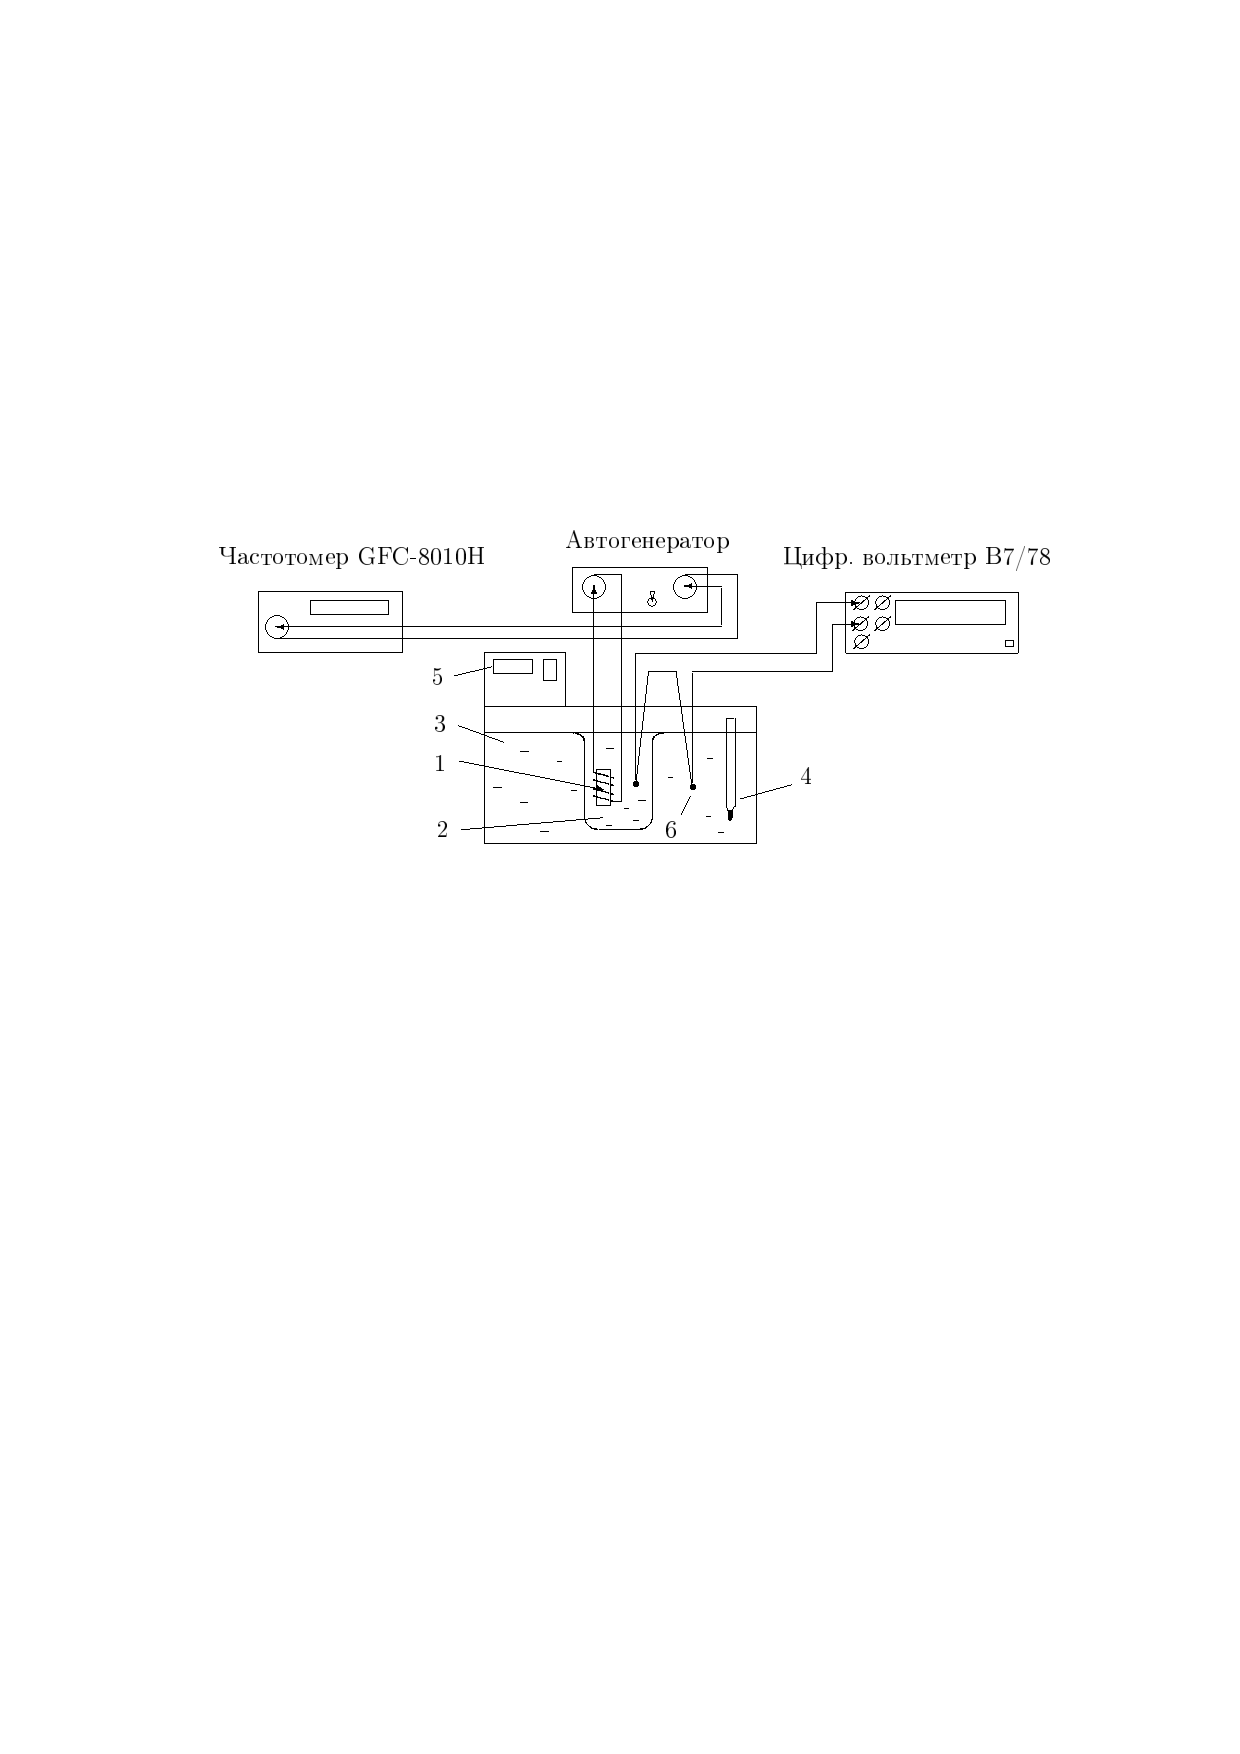
\includegraphics[scale=1]{inst.pdf}
		\end{figure}
	\section*{Ход работы}
		\begin{enumerate}
			\item Исследуем зависимость колебаний $ LC- $генератора от температуры образца, отмечая период колебаний $ \tau $ по частотомеру, а температуру $ T $ -- по показаниям термостата.
			\item Проведём измерения в диапазоне от $ 14\:^{\circ} C $ до $ 40\:^{\circ} C$ через $ 2\:^\circ C $.
		\end{enumerate}

	\section*{Обработка результатов}
		Полученные графики и таблицы представлены ниже:
		\begin{figure}[H]
			\label{2}
			\caption{Зависимость $ 1 /\left(\tau^{2}-\tau_{0}^{2}\right)=f(T) $}
			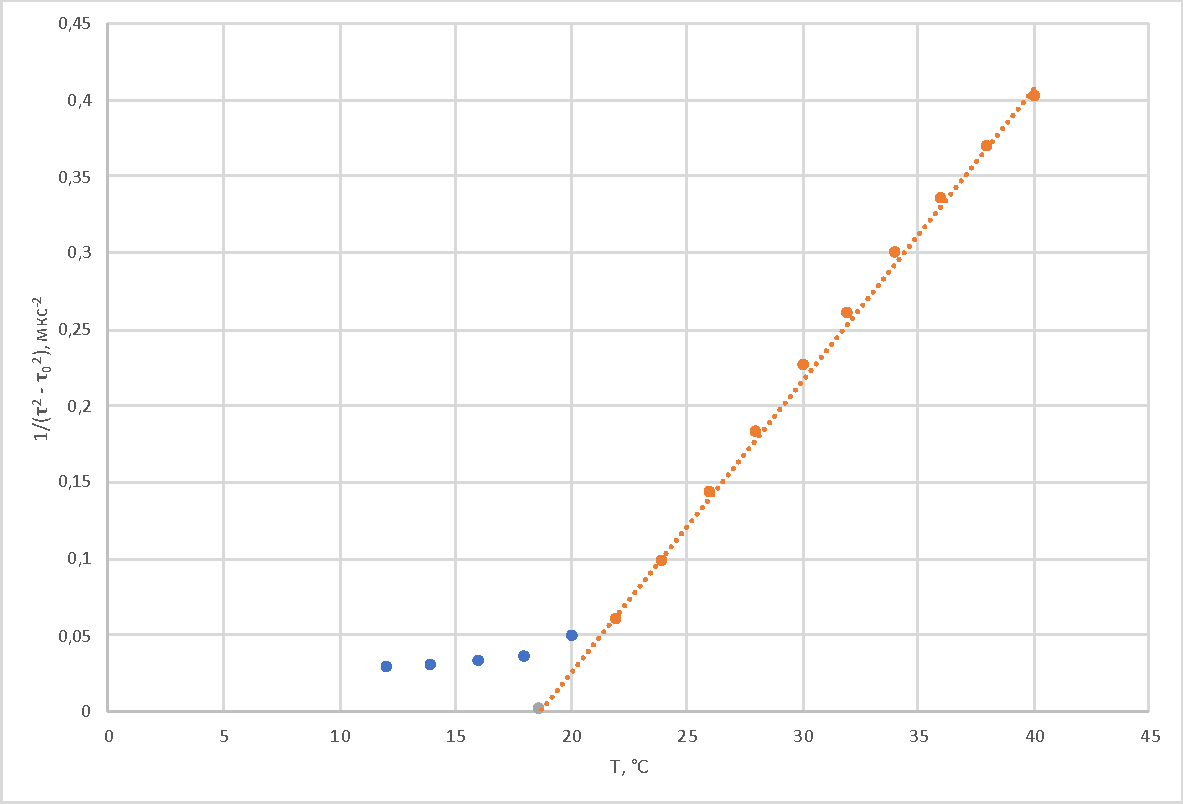
\includegraphics[scale=0.6]{2.pdf}
		\end{figure}
		
		\section*{Вывод}
			Таким образом, мы вычислили парамагнитную точку Кюри для гадолиния: $ \Theta_p=18,7\pm0,3\:^\circ C $. Табличное значение точки Кюри: $ T_C = 20,2\:^\circ C $ (Физические величины, справочник).
			
\end{document} % конец документа

